In der Bildverarbeitung kann ein gegebenes Signal häufig nur durch eine
unstetige Funktion dargestellt werden. Deshalb stellt sich zunächst die Frage,
welcher Funktionenraum zum Beschreiben dieser Signale geeignet ist.

Ist $\Omega\subset\Rbb^2$ ein beschränktes Lipschitz-Gebiet und $g:\Omega\to
\Rbb$ stellt ein gegebenes Signal auf $\Omega$ dar, so könnte $g$ im
Sobolev-Raum $W^{1,1}(\Omega)$ vermutet werden, da Elemente dieses Raums im
Allgemeinen nicht stetig sein müssen \cite[297]{Bar15}. 
Allerdings lassen Sobolev-Funktionen die oftmals benötigten Sprünge über
ein-kodimensionale Teilmengen von $\Omega$ nicht zu \cite[393]{ABM14}.
Dieses Problem kann gelöst werden, indem der Raum der Funktionen von
beschränkter Variation $\BV(\Omega)$ betrachtet wird. Dieser ist eine echte
Obermenge von $W^{1,1}(\Omega)$ und hat sich als geeignet für die Modellierung 
von Signalen in der Bildverarbeitung und weitere Anwendungen erwiesen (cf.
\cites[393]{ABM14}[42]{AK06}[297]{Bar15}[S. 1 f.]{Bra98}).

Eine mögliche Problemstellung in der Bildverarbeitung ist die 
Rauschunterdrück\-ung, das heißt der Versuch unerwünschtes Rauschen in einem
Signal zu verringern.
In \cite{ROF92} beschrieben Rudin, Osher und Fatemi 1992 ein
Modell-Problem dafür, welches deshalb als ROF-Modell bezeichnet wird (cf.
\cites[1217]{Bar15a}[132]{CP10}[S. 74 f.]{Get12}).
Dabei ist für das gegebene Signal $g\in L^2(\Omega)$ und 
eine Funktion $v\in\BV(\Omega)\cap L^2(\Omega)$ die Minimierung
von zwei Termen relevant.
Der erste Term ist die
Seminorm $|v|_{\BV(\Omega)}$ von $v$ auf $\BV(\Omega)$, die der
totalen Variation der distributionellen Ableitung $Dv$ von $v$ entspricht,
falls $v\in W^{1,1}(\Omega)$ mit der Seminorm auf $W^{1,1}(\Omega)$
übereinstimmt und deren Minimierung Oszillation verhindert aber Unstetigkeiten
zulässt \cite[72]{Get12}. Der zweite Term misst den Unterschied von $v$ und $g$ in 
$L^2(\Omega)$.
Damit und mit einen Parameter
$\alpha\in\Rbb_+$, der das Verhältnis zwischen Rauschverminderung und
Ähnlichkeit der Lösung zum Eingangssignal gewichtet, sucht das ROF-Modell
eine Funktion $u\in\BV(\Omega)\cap L^2(\Omega)$, die das Funktional
\begin{align*}
  I(v)\coloneqq |v|_{\BV(\Omega)}+\frac{\alpha}{2}\Vert
  v-g\Vert_{L^2(\Omega)}^2
\end{align*}
unter allen $v\in\BV(\Omega)\cap L^2(\Omega)$ minimiert.

Wird hierbei $\alpha$ zu klein gewählt, führt das zu einer zu stark
geglätteten, verwaschen aussehenden Lösung, zu sehen zum Beispiel in den
Abbildungen \ref{fig:snr10alpha100} und \ref{fig:snr10alpha1000}, während das
Rauschen im Vergleich zum Eingangssignal $g$ kaum verringert wird, falls
$\alpha$ zu groß gewählt wird, zu sehen zum Beispiel in den Abbildungen
\ref{fig:snr10alpha5000} und \ref{fig:snr10alpha10000}.

Für weitere Details und Referenzen zur Rauschunterdrückung und zur Wahl von
$\alpha$ siehe \cite{Get12}.

\medskip
--------------------------------
\medskip

Was wurde bisher gemacht für dieses PRoblem. 
übergang zu Bartels und Courant, was im folgenden weitergeht

\medskip
--------------------------------
---`\cite[Kapitel~10.1.3]{Bar15}
\medskip

In \cite[Kapitel 10]{Bar15} wird zur Diskretisierung des
ROF-Modell die Courant Finite-Elemente-Methode genutzt und eine primale-duale
Iteration zur numerischen Lösung verwendet.

In dieser Arbeit möchten wir die Konvergenzeigenschaften eines adaptiven
Algorithmus untersuchen, bei dem wir die primale-duale Iteration auf jedem
Level anwenden auf eine nichtkonforme Formulierung des ROF-Modells und eine
Diskretisierung mit der Crouzeix-Raviart Finite-Elemente Methode.
Dafür verwenden wir einen von Prof. Carstens zur Verfügung gestellten 
Verfeinerungsindikator. Die Implemtation basiert auf \cite{Car09a}.
Dabei sei angemerkt, dass wir folgende, leicht andere Formulierung des 
ROF-Modells betrachten. Wir minimieren das Funktional
\begin{align*}
  E(v)\coloneqq \frac{\alpha}{2}\Vert v\Vert_{L^2(\Omega)}^2 + |v|_{\BV(\Omega)}
  +\Vert v\Vert_{L^1(\partial\Omega)}-\int_\Omega fv\dx
\end{align*}
unter allen $v\in\BV(\Omega)\cap L^2(\Omega)$.
Für $f = \alpha g$ und alle $v\in \BV(\Omega)\cap
L^2(\Omega)$ gilt dann $I(v) =
E(v) - \Vert v\Vert_{L^1(\partial \Omega)}+ \frac{\alpha}{2}\Vert
g\Vert_{L^2(\Omega)}^2$. 
Der Zusammenhang mit dem ROF-Modell ist, aufgrund der Konstanz des Terms
$\frac{\alpha}{2}\Vert g\Vert_{L^2(\Omega)}^2$, folglich, dass die Funktionale
$E$ und $I$ die gleichen Minimierer in $\left\{v\in\BV(\Omega)\cap
L^2(\Omega)\mid \Vert v\Vert_{L^1(\partial\Omega)}=0\right\}$ besitzen.

Außerdem erlaubt uns die nichtkonforme Formulierung die Betrachtung einer
garantierten unteren Energieschranke.

\medskip
--------------------------------
\medskip

Dafür wird, nachdem in \Cref{chap:theoreticalBasics} zunächst die Notationen
eingeführt und die theoretischen Grundlagen aus der Optimierung und zu den
Funktionen beschränkter Variation zusammengetragen wurden, in
\Cref{chap:continuousProblem} bewiesen, dass für unsere Formulierung des
ROF-Modells ein eindeutiger
Minimierer existiert.
Anschließend folgt in \Cref{chap:discreteProblem} die nichtkonforme Formulierung
und Diskretisierung des Minimierungsproblems. Mithilfe eines
äquivalenten Sattelpunktsproblems werden äquivalente Charakterisierung, 
Existenz und Eindeutigkeit für den diskreten Minimierer bewiesen. Außerdem
werden die zu untersuchenden Konvergenzraten, der Verfeinerungsindikator und
die garantierte untere Energieschranke aufgeührt.
In \Cref{chap:algorithm} wird die primale-duale Iteration formuliert und bewiesen,
dass diese gegen den diskreten Minimierer konvergiert. 
Es folgen Hinweise zur Benutzung des Programm und Details zur Implementation
des Algorithmus in \Cref{chap:implementation} und schließlich in
\Cref{chap:experiments} die Darstellung der Experimente und deren Auswerung in
\Cref{chap:review}.


\begin{figure}[h]
  \centering
  \begin{subfigure}[b]{.4\linewidth}
    \caption{\url{https://homepages.cae.wisc.edu/~ece533/images/cameraman.tif}}
    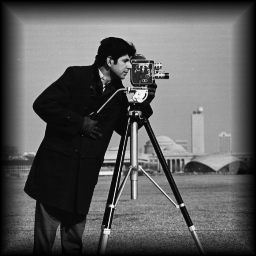
\includegraphics[width=\linewidth]{pictures/introBeta/cameraman.png}
    \label{fig:camerman}
  \end{subfigure}
  \quad
  \begin{subfigure}[b]{.4\linewidth}
    \caption{$\snr=10$}
    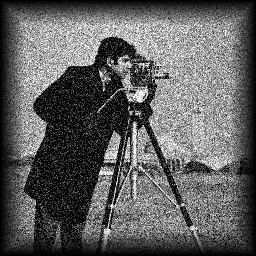
\includegraphics[width=\linewidth]{pictures/introBeta/snr10.png}
    \label{fig:camermanSNR10}
  \end{subfigure}

  \begin{subfigure}{.3\linewidth}
    \caption{$\alpha=100$}
    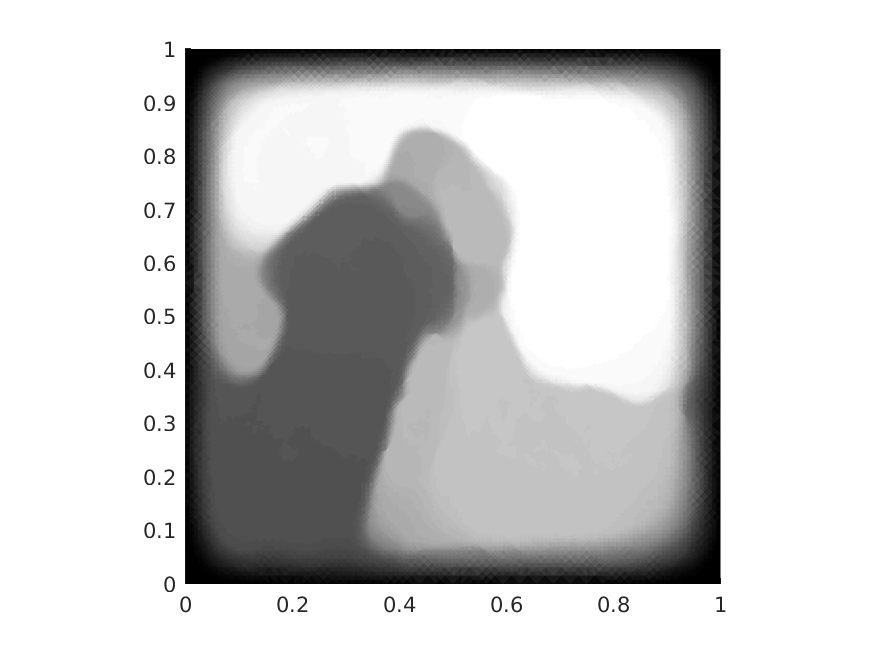
\includegraphics[trim = 60 0 60 20, clip, width=\linewidth]
      {pictures/introBeta/snr10/00100.png}
    \label{fig:snr10alpha100}
  \end{subfigure}
  \begin{subfigure}{.3\linewidth}
    \caption{$\alpha=1000$}
    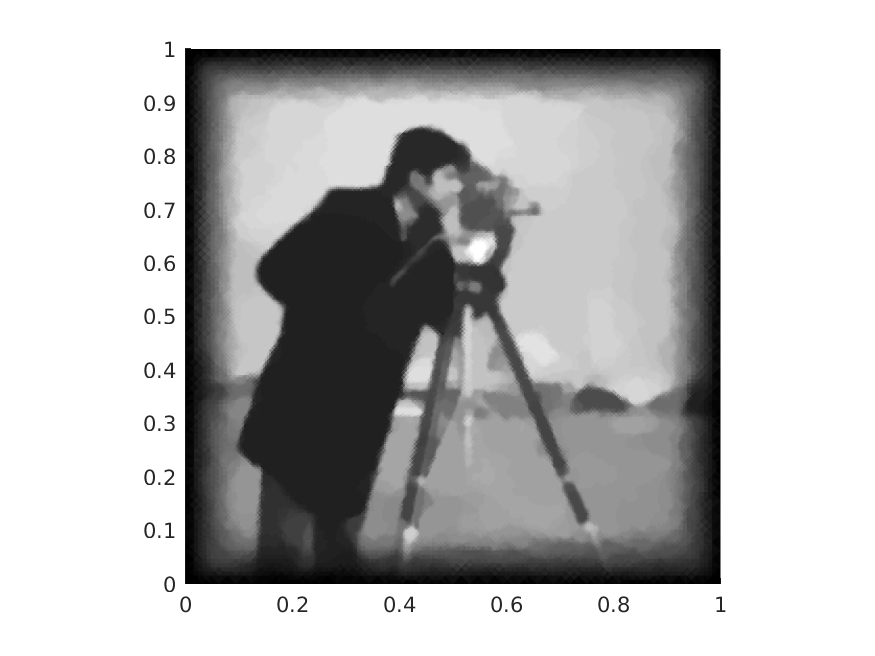
\includegraphics[trim = 60 0 60 20, clip, width=\linewidth]
      {pictures/introBeta/snr10/01000.png}
    \label{fig:snr10alpha1000}
  \end{subfigure}
  \begin{subfigure}{.3\linewidth}
    \caption{$\alpha=2500$}
    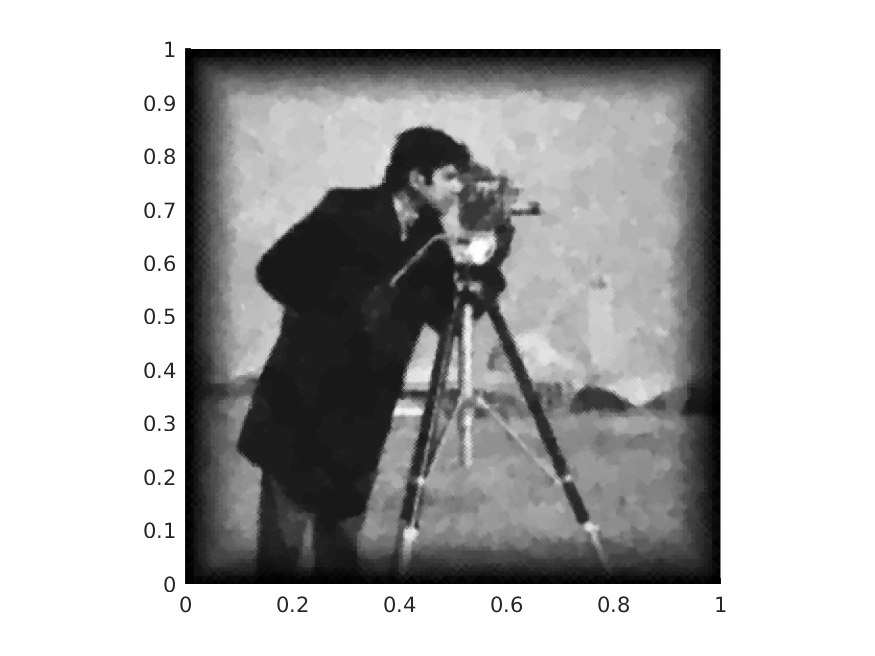
\includegraphics[trim = 60 0 60 20, clip, width=\linewidth]
      {pictures/introBeta/snr10/02500.png}
    \label{fig:snr10alpha2500}
  \end{subfigure}

  \begin{subfigure}{.3\linewidth}
    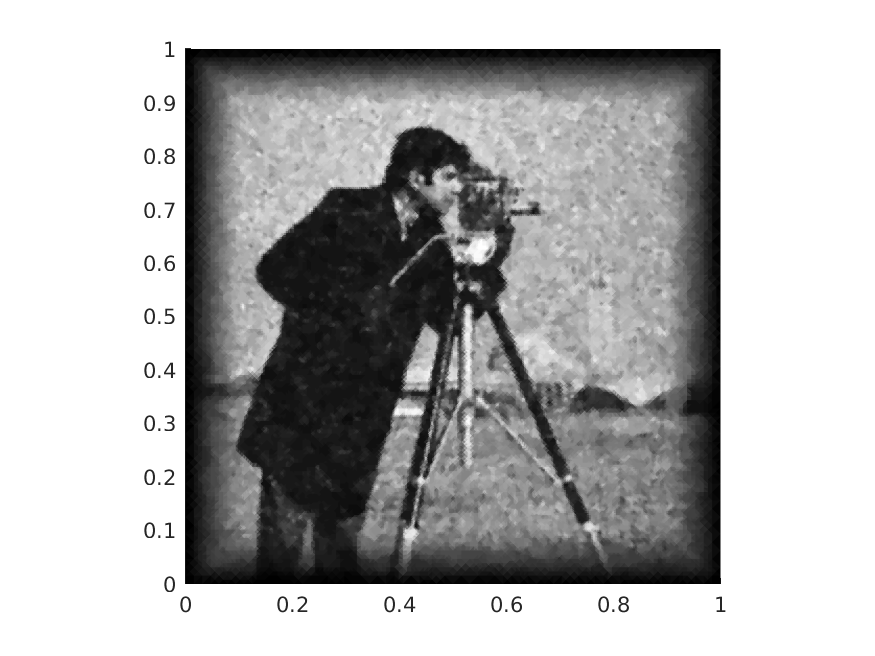
\includegraphics[trim = 60 0 60 20, clip, width=\linewidth]
      {pictures/introBeta/snr10/05000.png}
    \caption{$\alpha=5000$}
    \label{fig:snr10alpha5000}
  \end{subfigure}
  \begin{subfigure}{.3\linewidth}
    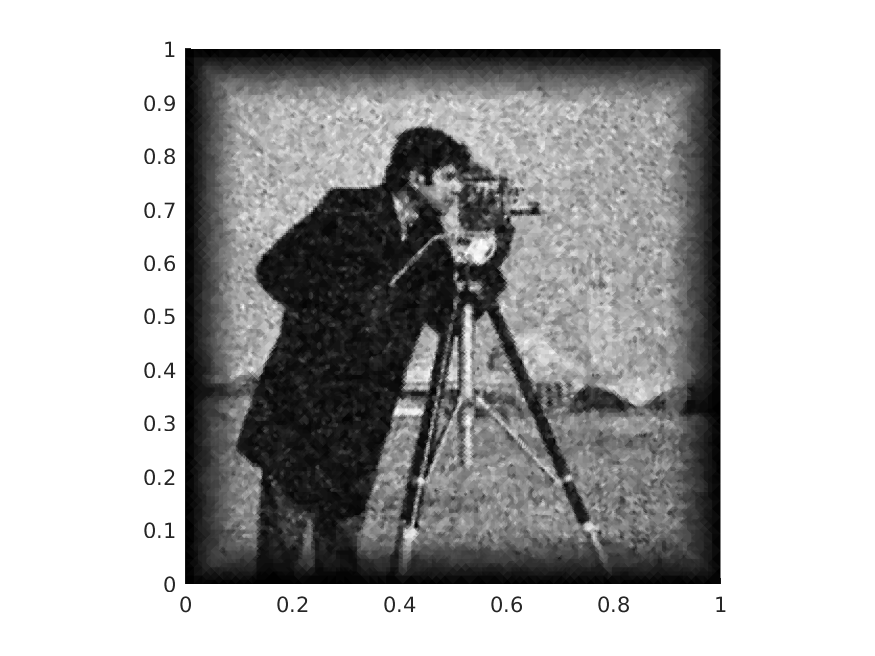
\includegraphics[trim = 60 0 60 20, clip, width=\linewidth]
      {pictures/introBeta/snr10/10000.png}
    \caption{$\alpha=10000$}
    \label{fig:snr10alpha10000}
  \end{subfigure}
  \caption{Originalbild (a) und Originalbild mit additiven weißen gaußschen
  Rauschen (b) mit einem Signal-Rausch-Verhältnis (eng.\ signal-to-noise
  ratio, SNR) von 10, jeweils mit nachträglich hinzugefügten graduellen
  Übergang zu schwarzen Rand, was Nullranddaten entspricht und drei Ergebnisse
  (c)-(g) des adaptiven Algorithmus mit verschiedenen Werten von $\alpha$}
  \label{fig:exampleDenoising}
\end{figure}

\todo[inline]{Experimente länger rechnen und vielleicht 9 Wahlen für alpha mit
einem ernsthaften Versuch, ein gut aussehendes entrauschtes Bild zu bekommen}
